%!TEX program = lualatex
\documentclass{report}
\usepackage[vietnamese]{babel}
\usepackage{hyperref}
\usepackage[acronym, toc]{glossaries}
\usepackage{graphicx}
\usepackage{fontspec}
\usepackage{titlesec}
\usepackage{fontsize}
\usepackage{xcolor}
\usepackage{caption}
\usepackage{subcaption}
\usepackage{float}
\usepackage{blindtext}
\usepackage{listingsutf8}
\usepackage{tikz}
\usepackage{fancyhdr}
\usepackage{indentfirst}

\changefontsize[20pt]{14pt}
\usepackage[
  paper=a4paper,
  left=30mm,
  right=20mm,
  top=25mm,
  bottom=25mm]{geometry}

\setmainfont{Times New Roman}

\titleformat{\chapter}[hang]
    {\normalfont\fontsize{16}{19}\bfseries}
    {Chương\ \thechapter:}
    {1em}
    {} 

\titleformat{\section}
    {\normalfont\fontsize{15}{19}\bfseries}
    {\thesection}
    {1em}
    {}
\titleformat{\subsection}
    {\normalfont\fontsize{14}{19}\bfseries\slshape}
    {\thesubsection}
    {1em}
    {}
\titleformat{\subsubsection}
    {\normalfont\fontsize{14}{19}\slshape}
    {\thesubsubsection}
    {1em}
    {}

\makenoidxglossaries

\newglossaryentry{latex}{
	name=Latex,
	description={Is a mark up language specially suited for scientific documents}
}

\newacronym{mcu}{VĐK}{vi điều khiển}
\newacronym{i2c}{I$^2$C}{Inter-Integrated Circuit}
\newacronym{uart}{UART}{Universal Asynchronous Receiver-Transmitter}
\newacronym{usart}{USART}{Universal Synchronous Asynchronous Receiver-Transmitter}
\newacronym{arm}{ARM}{Advanced RISC Machine}
\newacronym{usb}{USB}{Universal Serial Bus}
\newacronym{spi}{SPI}{Serial Peripheral Interface}
\newacronym{dma}{DMA}{Direct Memory Accecss}
\newacronym{adc}{ADC}{Analog to Digital Converter}

\lstset{basicstyle=\ttfamily, numbers=left, numberstyle=\small, numbersep=8pt, frame = single, breaklines=true}

\pagestyle{fancy}
\renewcommand{\chaptermark}[1]{\markboth{#1}{#1}}
\fancyhead[R]{}
\fancyhead[L]{\leftmark}

\widowpenalties 1 10000
\raggedbottom

\begin{document}

\begin{titlepage}
	
	\begin{center}
		\begin{tikzpicture}[remember picture,overlay,inner sep=0,outer sep=0]
		     \draw[blue!70!black,line width=4pt]
		     ([xshift=-1.5cm,yshift=-2cm]current page.north east) coordinate (A)--
		     ([xshift=2.5cm,yshift=-2cm]current page.north west) coordinate(B)--
		     ([xshift=2.5cm,yshift=2cm]current page.south west) coordinate (C)--
		     ([xshift=-1.5cm,yshift=2cm]current page.south east) coordinate(D)--
		     cycle;
		\end{tikzpicture}
		
		\textbf{HỌC VIỆN KỸ THUẬT MẬT MÃ}
		
		KHOA CÔNG NGHỆ THÔNG TIN
		
		\vspace{1cm}
		
		
\includegraphics[width=0.3\textwidth]{../images/kma.png}
		
		
		\vspace{2.2cm}
		
		\textbf{BÀI TẬP MÔN LẬP TRÌNH HỆ THỐNG NHÚNG LINUX}
		
		\vspace{0.2cm}
		
		\color{red}
		\textbf{XÂY DỰNG ỨNG DỤNG VỚI GIAO DIỆN ĐỒ HỌA NHẬP VÀO DÒNG KÝ TỰ, SAU ĐÓ HIỂN THỊ DÒNG KÝ TỰ ĐÓ LÊN MÀN HÌNH LCD VÀ GIAO DIỆN ỨNG DỤNG}
		
		
		
	\end{center}

	\begin{flushleft}        
		\hspace{3cm}
		Khoa: Công nghệ thông tin
		
		\hspace{3cm}
		Chuyên ngành: Kỹ thuật phần mềm nhúng và di động
		
		
		\vfill
		
		\hspace{3cm}
		
		\hspace{3cm}Người hướng dẫn
		
		\begin{tabular}{l c}
			
			\hspace{4cm}\textbf{ThS. Lê Thị Hồng Vân} \\
			\hspace{4cm}{Khoa công nghệ thông tin - Học viện Kỹ thuật Mật mã}
			
			
		\end{tabular}
		
		\vspace{0.5cm}
		
		\hspace{3cm}Nhóm sinh viên thực hiện:
		
		\begin{tabular}{l c c}
			
			\hspace{4cm}Phạm Văn Dũng & CT040308 \\
						
			\hspace{4cm}Phạm Thị Phương Anh & CT040401 \\
			
			\hspace{4cm}Nhóm 01
			
			
		\end{tabular}
		
	\end{flushleft}
	
	\begin{center}
		
		\vspace{1cm}
		
		Hà Nội - 2023
		
	\end{center}
\end{titlepage}

\pagenumbering{roman}

\renewcommand{\contentsname}{MỤC LỤC}
\renewcommand{\listfigurename}{DANH SÁCH HÌNH VẼ}
\renewcommand{\listtablename}{DANH SÁCH BẢNG}

\cleardoublepage
\phantomsection
\addcontentsline{toc}{chapter}{MỤC LỤC}


\tableofcontents

\cleardoublepage
\phantomsection
\addcontentsline{toc}{chapter}{DANH SÁCH HÌNH VẼ}

\listoffigures

\cleardoublepage
\phantomsection
\addcontentsline{toc}{chapter}{DANH SÁCH BẢNG}

\listoftables

\printnoidxglossary[title=DANH MỤC TỪ VIẾT TẮT, toctitle=DANH SÁCH TỪ VIẾT TẮT, type=\acronymtype]

\chapter*{LỜI NÓI ĐẦU}
\phantomsection
\addcontentsline{toc}{chapter}{LỜI NÓI ĐẦU}


Các hệ thống nhúng đã hiện diện trong hầu hết các hoạt động của con người trong cuộc sống ngày nay, từ các thiết bị điện đơn giản đến các thiết bị phức tạp. Phát triển các hệ thống nhúng như vậy, yêu cầu lượng thời gian nghiên cứu cũng như lượng kiến thức lớn gấp bội khi độ phức tạp của hệ thống tăng lên. Để đơn giản hóa quy trình phát triển cũng như chi phí xây dựng hệ thống, các hệ thống nhúng nói trên có thể phát triển trên nền hệ điều hành linux.


Với mong muốn tìm hiểu sâu hơn về hệ sinh thái mã nguồn mở linux và quy trình phát triển hệ thống nhúng trên nền linux, nhóm chúng em quyết định thực hiện đề tài: “\textbf{Xây dựng ứng dụng với giao diện đồ họa nhập vào dòng ký tự, sau đó hiển thị dòng ký tự đó lên màn hình LCD và giao diện ứng dụng}”. Báo cáo bao gồm các chương và bố cục sau:

\hspace{1cm}Chương 1: Cơ sở lý thuyết

\hspace{1cm}Chương 2: Phân tích - Thiết kế

\hspace{1cm}Chương 3: Xây dựng hệ thống

\hspace{1cm}Chương 4: Kết luận

\vspace{0.5cm}

\hspace{6cm}Hà Nội, ngày 06 tháng 6 năm 2022

\vspace{2cm}

\hspace{7cm}Nhóm sinh viên thực hiện

\newpage

\pagenumbering{arabic}

\chapter{CƠ SỞ LÝ THUYẾT}
\section{Hệ thống nhúng}
\subsection{Khái niệm hệ thống nhúng}

Hệ thống nhúng (Embedded system) là một thuật ngữ để chỉ một hệ thống có khả năng tự trị được nhúng vào một môi trường hay một hệ thống mẹ. Đó là các hệ thống tích hợp cả phần cứng và phần mềm phục vụ các bài toán chuyên dụng trong nhiều lĩnh vực công nghiệp, tự động hoá điều khiển, quan trắc và truyền tin. Đặc điểm của các hệ thống nhúng là hoạt động ổn định và có tính năng tự động hoá cao. \cite{giao-trinh}

Hệ thống nhúng thường được thiết kế để thực hiện một chức năng chuyên biệt nào đó. Khác với các máy tính đa chức năng, chẳng hạn như máy tính cá nhân, một hệ thống nhúng chỉ thực hiện một hoặc một vài chức năng nhất định, thường đi kèm với những yêu cầu cụ thể và bao gồm một số thiết bị máy móc và phần cứng chuyên dụng mà ta không tìm thấy trong một máy tính đa năng nói chung. Vì hệ thống chỉ được xây dựng cho một số nhiệm vụ nhất định nên các nhà thiết kế có thể tối ưu hoá nó nhằm giảm thiểu kích thước và chi phí sản xuất. Các hệ thống nhúng thường được sản xuất hàng loạt với số lượng lớn. Hệ thống nhúng rất đa dạng, phong phú về chủng loại. Xét về độ phức tạp, hệ thống nhúng có thể rất đơn giản với một vi điều khiển hoặc rất phức tạp với nhiều đơn vị, các thiết bị ngoại vi và mạng lưới được nằm gọn trong một lớp vỏ máy lớn.

Các thiết bị PDA hoặc máy tính cầm tay cũng có một số đặc điểm tương tự với hệ thống nhúng như các hệ điều hành hoặc vi xử lý điều khiển chúng nhưng các thiết bị này không phải là hệ thống nhúng thật sự bởi chúng là các thiết bị đa năng, cho phép sử dụng nhiều ứng dụng và kết nối đến nhiều thiết bị ngoại vi.

Có rất nhiều hãng sản xuất bộ vi xử lý và phần cứng khác nhau: Texas Instrument, Freescale, ARM, Intel, Motorola, Atmel, AVR, …

Những hệ điều hành khác nhau: QNX, ulTRON, Windows CE/XP Embedded, Embedded Linux, …

Những ngôn ngữ lập trình khác nhau: C/C++, Assembly, PLC, …

\subsection{Cấu trúc hệ thống nhúng}

Vơ bản thì cấu trúc của hệ thống nhúng sẽ bao gồm 3 phần: phần mềm hệ thống, phần mềm ứng dụng, bộ vi xử lý.

Phần mềm hệ thống: phần mềm này không bắt buộc phải có và có thể tái sử dụng trên một hệ thống nhúng khác. Chúng có chức năng quản lý bộ nhớ, quản lý tiến trình, quản lý chia sẻ tài nguyên. Trình điều khiển thiết bị: \acrshort{uart}, Ethernet, \acrshort{adc}… Hệ điều hành nhúng: eCos, ucLinux, VxWorks, Monta Vista Linux, BIOS, QNX…

Phần mềm ứng dụng: không bắt buộc phải có và khó tái sử dụng trên một hệ thống nhúng khác. Chúng có chức năng quyết định hành vi cho một hệ thống nhúng.

Bộ vi xử lý (Hardware): đây là các thành phần bắt buộc trong một hệ thống nhúng, gồm có một số thiết bị như vi xử lý, bộ nhớ, tụ điện, điện trở, mạch tích hợp, bản in mạch,…

\begin{figure}[H]
	\centering
	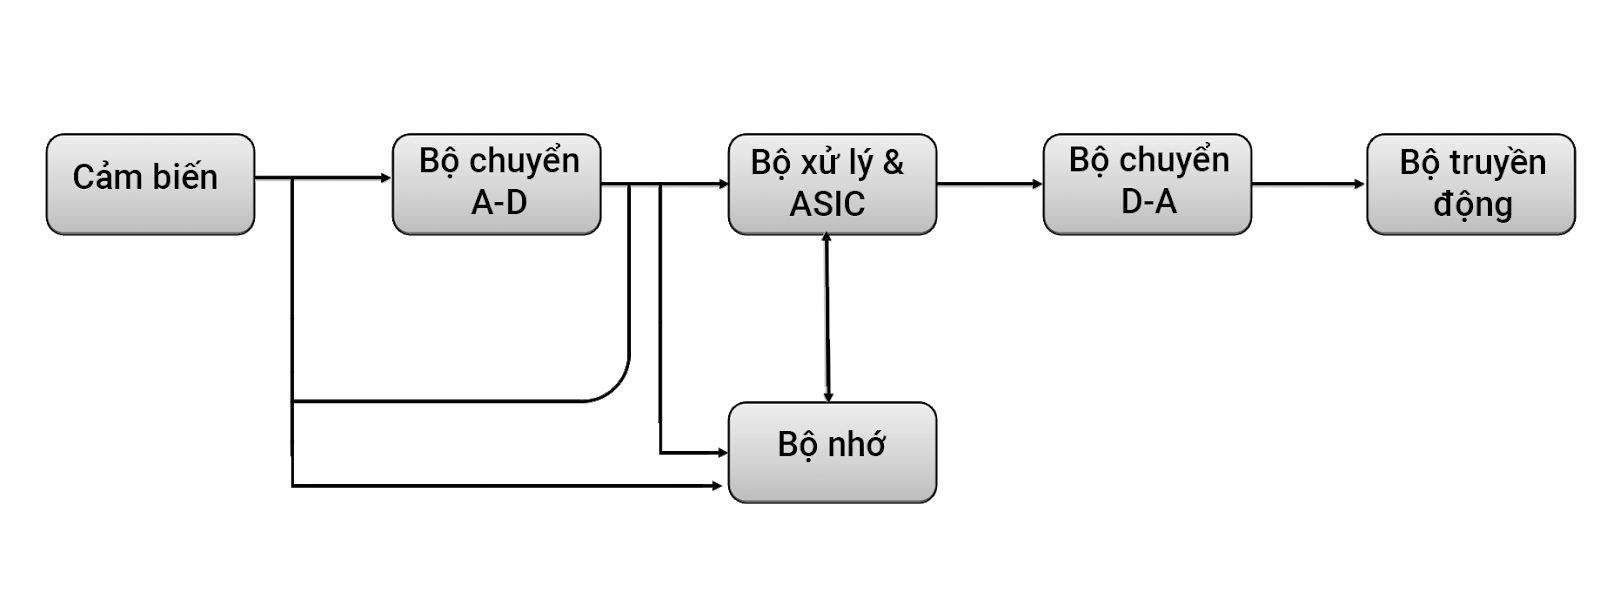
\includegraphics[width=0.8\textwidth]{../images/cau-truc-he-thong-nhung.png}
	\caption{Cấu trúc hệ thống nhúng}
\end{figure}

\subsection{Phát triển phần mềm trong hệ thống nhúng}
Một hệ thống nhúng luôn có 3 thành phần:
\begin{itemize}
	\item Hardware (Phần cứng): Là phần quan trọng nhất của hệ thống nhúng, nó quyết định chính đến chất lượng, giá thành của hệ thống nhúng.
	\item Operation System (Hệ điều hành): Là phần mềm chạy đầu tiên trong hệ thống cho chức năng điều khiển, quản lý tài nguyên của hệ thống và cung cấp một giao diện phát triển chung.
	\item Applications (Phần mềm ứng dụng): Quyết định chức năng của hệ thống và là thành phần tương tác với người dùng. Trong Linux, nó được gọi là phần mềm nhúng Linux
\end{itemize}

Hệ điều hành nhúng Linux (Linux Embedded Software) là những hệ điều hành nhúng sử dụng nhân Linux, có chức năng điều khiển phần cứng hoặc thiết bị kết nối với hệ thống. Không giống với những phần mềm ứng dụng (Application Software) có thể chạy nhiều hệ thống máy tính, phần mềm nhúng Linux chỉ có thể chạy được trên những phần cứng cố định. Phần mềm nhúng Linux phải được thiết kế để chạy được trên những hệ thống hạn chế về tốc độ xử lý, bộ nhớ… mà vẫn đảm bảo hiệu năng.
\section{Hệ thống nhúng sử dụng hệ điều hành linux}
\subsection{Khái niệm hệ thống nhúng linux}

Linux là một hệ điều hành mã nguồn mở (Open-source OS) chạy trên hầu hết các kiến trúc vi xử lý, bao gồm dòng vi xử lý ARM. Linux được hỗ trợ bởi một cộng đồng mã nguồn mở (GNU), chính điều này làm cho Linux rất linh hoạt và phát triển rất nhanh với nhiều tính năng không thua kém các hệ điều hành khác hiện nay. Tất cả các ứng dụng chạy trên hệ điều hành UNIX đều tương thích với Linux.

Hầu hết các bản Linux đều hỗ trợ rất nhiều ngôn ngữ lập trình, đặc biệt công cụ GCC cho phép người lập trình có thể biên dịch và thực thi ứng dụng viết bằng nhiều ngôn ngữ lập trình khác nhau: C/C++, Java, .v.v... Ngoài ra, Linux còn hỗ trợ ngôn ngữ lập trình để phát triển các ứng dụng đồ họa như: JTK+, Qt, .v.v...

Do chi phí thấp, khả năng thay đổi tương thích với phần cứng dễ dàng nên nhúng Linux thường được sử dụng rất nhiều trong các hệ thống nhúng (embedded system). Ngày nay, Linux đã trở thành một đối thủ cạnh tranh lớn về lĩnh vực hệ điều hành trong các dòng điện thoại thông minh (smartphone), các thiết bị PDA (personal digital assistant) và là một lựa chọn thay thế cho sự độc quyền của Windows CE và Palm OS.

Theo định nghĩa của IEEE (Hiệp hội kỹ sư điện và điện tử Hoa kỳ): Hệ thống nhúng là một phần của hệ thống lớn hơn và thực hiện một số chức năng của hệ thống đó.

Đặc trưng của hệ điều hành nhúng:
\begin{itemize}
	\item Tăng tính tin cậy (reliability)
	\item Tăng tính khả chuyển (portability)
	\item Khả năng tương thích mềm: dễ dàng nâng cấp hay thu gọn để tương thích với nền tảng hệ thống
	\item Cung cấp các cơ chế lập lịch (scheduler) hỗ trợ thời gian thực (Realtime OS – RTOS)
\end{itemize}
\begin{figure}[H]
	\centering
	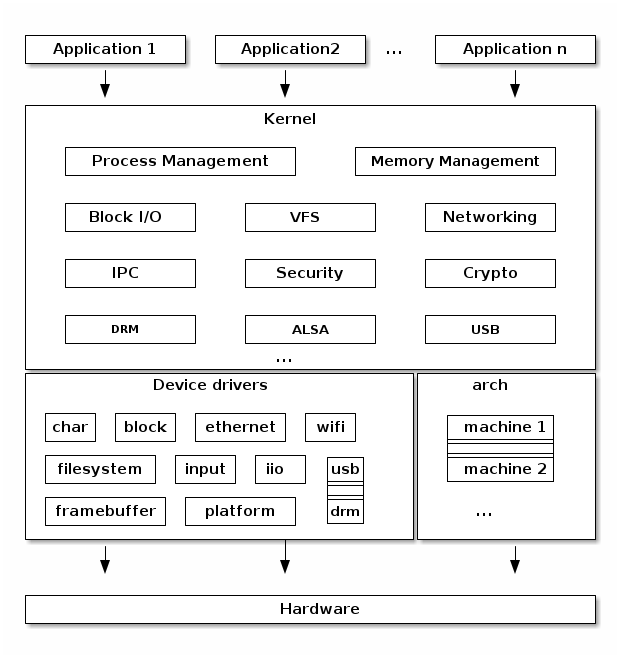
\includegraphics[width=0.8\textwidth]{../images/cau-truc-linux.png}
	\caption{Cấu trúc hệ điều hành}
\end{figure}

\subsection{Các thành phần trong hệ thống nhúng linux}
Nhân Linux (Linux Kernel): Nhân Linux là thành phần cốt lõi của hệ điều hành Linux. Nó quản lý tài nguyên phần cứng, quản lý bộ nhớ, giao tiếp với thiết bị và cung cấp các dịch vụ hệ thống cần thiết. Nhân Linux có thể được tùy chỉnh để phù hợp với các yêu cầu của hệ thống nhúng và được cung cấp bởi dự án Linux Kernel.

Bootloader: Bootloader là chương trình đầu tiên được chạy khi hệ thống được khởi động. Nó có nhiệm vụ khởi động và tải nhân Linux vào bộ nhớ và sau đó chuyển quyền kiểm soát cho nhân Linux. Các bootloader phổ biến cho hệ thống nhúng Linux bao gồm U-Boot và GRUB.

Thư viện hỗ trợ: Hệ thống nhúng Linux cung cấp các thư viện hỗ trợ như libc, libpthread, libm và nhiều thư viện khác. Những thư viện này cung cấp các hàm, giao diện và tài nguyên hỗ trợ cho việc phát triển ứng dụng.

Công cụ phát triển: Hệ thống nhúng Linux cung cấp các công cụ phát triển mạnh mẽ. Đây là thành phần quan trọng giúp biên dịch các chương trình C tới đúng định dạng nhị phân của hệ thống đích bao gồm:
\begin{itemize}
	\item Compiler: GNU C Compiler.
	\item C library: Bao gồm các header file cho phép giao tiếp với hệ điều hành.
	\item Gdb: Hỗ trợ gỡ lỗi.
	\item Hệ thống Makefile
\end{itemize}

Giao diện người dùng: Giao diện người dùng trong hệ thống nhúng Linux có thể được phát triển bằng sử dụng các framework như Qt hay GTK+. Các giao diện người dùng có thể được hiển thị trên màn hình, giao tiếp thông qua các thiết bị nhập liệu và hiển thị kết quả của ứng dụng.


\subsection{Lập trình ngoại vi trong hệ thống nhúng linux}
Trong Linux, việc lập trình các thiết bị ngoại vi có thể được thực hiện ở hai nơi khác nhau: trong không gian người dùng (user space) hoặc trong không gian nhân (kernel space). 

Viết chương trình trong không gian người dùng không đòi hỏi kiến thức sâu về hệ điều hành Linux và kernel. Chương trình trong không gian người dùng sử dụng các API, thư viện hoặc giao thức cung cấp bởi kernel để tương tác với thiết bị thông qua các giao tiếp như \acrshort{usb}, \acrshort{i2c}, GPIO. Chương trình dạng này không có quyền truy cập trực tiếp vào phần cứng và cần sự hỗ trợ từ driver đã được cài đặt trong kernel.

Viết driver trong không gian nhân yêu cầu kiến thức về lõi hệ điều hành Linux và cách thức hoạt động của thiết bị.
Driver trong không gian nhân được biên dịch thành mô-đun nhân và chạy trong không gian nhân. Chúng có quyền truy cập trực tiếp vào phần cứng và cung cấp các API để cho phép các ứng dụng trong không gian người dùng tương tác với thiết bị.
Viết driver trong không gian nhân có thể đòi hỏi quyền root (hoặc sử dụng sudo) để tải và cài đặt driver vào hệ thống.

Trong nhiều trường hợp, viết chương trình trong không gian người dùng là đủ để tương tác với các thiết bị ngoại vi trong Linux. Tuy nhiên, trong một số trường hợp đặc biệt hoặc khi yêu cầu tương tác phức tạp hơn, viết driver trong không gian nhân có thể là lựa chọn tốt hơn.

\subsection{Trình điều khiển thiết bị trong linux}

Linux kernel driver là một module được nạp vào nhân linux và chạy trên không gian địa chỉ của nhân linux giúp cung cấp các chức năng mở rộng cho nhân hệ điều hành.

Device driver trong linux là một kernel module cung cấp giao diện giao tiếp với các thiết bị phần cứng như \acrshort{usb}, PCI, \acrshort{i2c}, \acrshort{spi}, … Device driver thực hiện việc giao tiếp như gửi và nhận dữ liệu, từ thiết bị, đảm bảo cho thiết bị được hoạt động đúng mục đích đặt ra. \cite{tutorial}

 \subsection{Trình điều khiển thiết bị \acrshort{i2c}}

	Khác với các thiết bị như PCI hay \acrshort{usb}, thiết bị sử dụng giao tiếp \acrshort{i2c} mặc định không được nhận biết bởi phần cứng mà thay vào đó phần mềm phải nhận biết những thiết bị nào được kết nối ở địa chỉ nào. Có một số cách để thực hiện việc này nhưng một phương pháp hiệu quả là sử dụng Device tree. \cite{i2c-instance}

Device tree là một cấu trúc dsữ liệu và một hệ thống mô tả phần cứng được sử dụng trong hệ điều hành linux. Trong Device tree, các thiết bị \acrshort{i2c} được khai báo tại bus và địa chỉ xác định. Cùng với thông tin bus và địa chỉ, Device tree còn mô tả loại driver tương thích với thiết bị. Khi trình điều khiển thiết bị được nạp, hàm probe sẽ được gọi khi trình điều khiển tương thích với thiết bị được khai báo trong Device tree.

Một Device tree cho thiết bị slave I2C có cấu trúc dạng như sau: thiết bị i2c-device được kết nối tới i2c-bus có địa chỉ 0x50. Driver tương thích là “vendor,i2c-device":
\begin{lstlisting}
	i2c {
		compatible = "i2c-bus";
		#address-cells = <1>;
		#size-cells = <0>;
		i2c-device@50 {
			compatible = "vendor,i2c-device";
			reg = <0x50>;
		}
	}
\end{lstlisting}

Bên trong driver, sau khi hàm probe được gọi với tham số struct i2c\_client tương ứng, thực hiện lưu lại biến này để thực hiện giao tiếp với thiết bị. Để đọc từ i2c device, sử dụng hàm i2c\_smbus\_read*, và i2c\_smbus\_write* cho việc ghi.

\subsection{Giao tiếp với trình điều khiển thiết bị}

Một số lựa chọn để giao tiếp với device driver của thiết bị nhúng bao gồm:

\begin{itemize}
	\item Sử dụng Character device driver
	\item Sử dụng sysfs
	\item Kết hợp các phương pháp
\end{itemize}


Với character device driver thiết bị được xuất hiện trên không gian người dùng với một file duy nhất bên trong /dev. Các thao tác có thể được thực hiện thông qua các lời gọi từ struct file\_operations như open, close, read, write, ioctl. Thông qua device file, thiết bị dạng vào/ra sẽ đơn giản hơn thông qua các lời gọi hệ thống. Một số ứng dụng sử dụng device file bao gồm: Giao tiếp với cổng serial, đọc từ ổ đĩa, …

Khác với character device driver, ứng dụng có thể sử dụng sysfs cho việc thiết lập và quản lý cấu hình. Các file trong không gian người dùng xuất hiện dưới dạng thư mục trong /sys/kernel/. Bên trong thư mục này là các file cấu hình được tạo ra với device driver giúp chương trình trong không gian người dùng có thể tương tác với driver thông qua việc đọc ghi các file. Giao tiếp với thiết bị phần cứng sẽ dễ dàng hơn thông qua sysfs do phần cứng có nhiều tham số cần đọc và ghi và chúng được tách riêng chúng ra từng file.

Với phần cứng hỗ trợ cả cấu hình các tham số và vào ra lượng thông tin lớn, kết hợp cả character device driver và sysfs sẽ tận dụng được lợi thế của cả hai phương pháp. Các thao tác vào ra sẽ được thực hiện qua character device driver, các thao tác cấu hình sẽ được thực hiện thông qua hệ thống sysfs và thao tác ioctl của character device driver. Khi đó người dùng có thể làm quen với thiết bị thông qua sysfs và thực hiện các thao tác qua chúng. Khi lập trình, việc sử dụng character device driver sẽ đem lại hiệu quả cao hơn.

\subsection{Lập trình giao diện trong hệ thống nhúng linux}
Khi lập trình giao diện đồ họa trong hệ thống nhúng linux, việc lựa chọn công nghệ phổ biến sẽ giúp quá trình phát triển trở nên dễ dàng hơn với bộ thư viện hỗ trợ rộng lớn, hỗ trợ từ cộng đồng cũng nhiều hơn.

Qt là một framework phát triển ứng dụng đa nền tảng rất mạnh mẽ và phổ biến. Nó cung cấp các công cụ và thư viện để phát triển giao diện người dùng, bao gồm cả hỗ trợ cho các thiết bị nhúng. Lập trình viên có thể sử dụng Qt để xây dựng giao diện người dùng đẹp và tương tác trong hệ thống nhúng Linux.

Qt được sử dụng để phát triển giao diện người dùng đồ họa (GUI) và các ứng dụng đa nền tảng chạy trên tất cả các nền tảng máy tính để bàn lớn và hầu hết các nền tảng di động hoặc nhúng. Hầu hết các chương trình GUI được tạo bằng Qt đều có giao diện tự nhiên, trong trường hợp này Qt được phân loại là widget toolkit. Ngoài ra các chương trình không phải GUI cũng có thể được phát triển, chẳng hạn như các công cụ dòng lệnh và consoles cho server. Một ví dụ về một chương trình không phải GUI sử dụng Qt là khung công tác web Cutelyst.

Qt hỗ trợ các trình biên dịch khác nhau, bao gồm trình biên dịch GCC C++ và bộ Visual Studio và có hỗ trợ quốc tế hóa rộng rãi. Qt cũng cung cấp Qt Quick, bao gồm một ngôn ngữ kịch bản lệnh được gọi là QML cho phép sử dụng JavaScript hoặc nhiều ngôn ngữ khác để cung cấp logic. Với Qt Quick, việc phát triển ứng dụng nhanh chóng cho các thiết bị di động trở nên khả thi, trong khi logic vẫn có thể được viết bằng mã gốc để đạt được hiệu suất tốt nhất có thể.

Các tính năng khác bao gồm truy cập cơ sở dữ liệu SQL, phân tích cú pháp XML, phân tích cú pháp JSON, quản lý luồng và hỗ trợ mạng. 

Một số lợi thế của bộ công cụ QT:
\begin{itemize}
	\item Phát triển đa nền tảng: Qt cho phép nhà phát triển viết mã một lần và triển khai trên nhiều nền tảng, bao gồm Windows, macOS, Linux, Android và iOS.
	
	\item Qt Widgets và Qt Quick: Qt cung cấp hai phương pháp chính để xây dựng giao diện người dùng. Qt Widgets là một framework trưởng thành và mạnh mẽ để tạo ra các ứng dụng trên máy tính để bàn, trong khi Qt Quick là một framework hiện đại và khai báo để tạo ra giao diện người dùng mượt mà và linh hoạt, phù hợp cho các nền tảng di động và nhúng.
	
	\item Tín hiệu và khe cắm: Cơ chế tín hiệu và khe cắm của Qt cho phép lập trình dựa trên sự kiện, giúp kết nối các phần khác nhau của ứng dụng và phản ứng với hành động người dùng hoặc sự kiện hệ thống.
	
	\item Thư viện phong phú: Qt cung cấp một loạt thư viện và mô-đun, bao gồm hỗ trợ cho giao tiếp mạng, phân tích XML, tích hợp cơ sở dữ liệu (Qt SQL), đa phương tiện (Qt Multimedia), đồ họa 2D/3D (Qt Graphics View) và nhiều hơn nữa.
	
	\item Môi trường phát triển tích hợp (IDE): Qt cung cấp một môi trường phát triển tích hợp được gọi là Qt Creator, cung cấp các tính năng như chỉnh sửa mã, gỡ lỗi, quản lý dự án và một trình thiết kế giao diện người dùng đồ.
\end{itemize}

\section{Các thiết bị ngoại vi}
\subsection{Máy tính nhúng Raspberry pi 3}
Raspberry Pi 3 là một bo mạch nhúng mạnh mẽ và phổ biến được sử dụng rộng rãi trong các ứng dụng nhúng. Một số lợi thế khi sử dụng Raspberry Pi 3 cho các ứng dụng nhúng:

\begin{enumerate}
	\item Hiệu suất mạnh mẽ: Raspberry Pi 3 được trang bị bộ vi xử lý ARM Cortex-A53 64-bit tốc độ 1.2GHz và RAM 1GB, mang lại khả năng xử lý nhanh và hiệu suất cao cho các ứng dụng đòi hỏi.
	
	\item Kết nối đa dạng: Raspberry Pi 3 có sẵn các cổng kết nối như HDMI, Ethernet, \acrshort{usb}, Bluetooth và Wi-Fi, cho phép kết nối dễ dàng với các thiết bị ngoại vi và mạng.
	
	\item GPIO (General Purpose Input/Output): Raspberry Pi 3 có giao diện GPIO cho phép tương tác với các linh kiện ngoại vi như cảm biến, động cơ và đèn LED. Điều này cho phép bạn tạo ra các ứng dụng nhúng tùy chỉnh và điều khiển các thiết bị ngoại vi khác.
	
	\item Hỗ trợ hệ điều hành Linux: Raspberry Pi 3 hỗ trợ nhiều hệ điều hành Linux như Raspbian, Ubuntu và các biến thể khác. Điều này giúp dễ dàng phát triển và triển khai ứng dụng nhúng dựa trên các công cụ và thư viện mạnh mẽ của Linux.
	
	\item Cộng đồng phát triển mạnh mẽ: Raspberry Pi có một cộng đồng phát triển đông đảo và nhiều tài liệu hướng dẫn, ví dụ như tài liệu phần cứng, tài liệu lập trình và diễn đàn. Điều này giúp giảm thời gian phát triển và tìm kiếm giải pháp cho các vấn đề gặp phải.
	
	\item Giá cả phải chăng: Raspberry Pi 3 có giá thành khá thấp so với nhiều bo mạch nhúng khác trên thị trường. Điều này giúp nó trở thành lựa chọn phổ biến cho các dự án nhúng có ngân sách hạn chế.
\end{enumerate}

Như vậy, có thể thấy rằng Raspberry pi là một bo mạch nhúng mạnh mẽ và đa năng, thích hợp cho nhiều ứng dụng nhúng như Internet of Things (IoT), hệ thống điều khiển nhúng và các dự án cá nhân. 
\subsection{Mô đun màn hình LCD 1602 HD44780}

Màn hình LCD1602 là màn hình ma trận điểm với 2 hàng, mỗi hàng chứa 16 ký tự kích thước 5x8 điểm. HD44780 là một IC điều khiển màn hình ma trận 5x8 hoặc 5x10 với tối đa 80 ký tự, phù hợp với màn hình LCD1602. Việc điều khiển yêu cầu tối thiểu 6 chân GPIO. Các bước khởi tạo màn hình.


\begin{figure}[H]
	\centering
	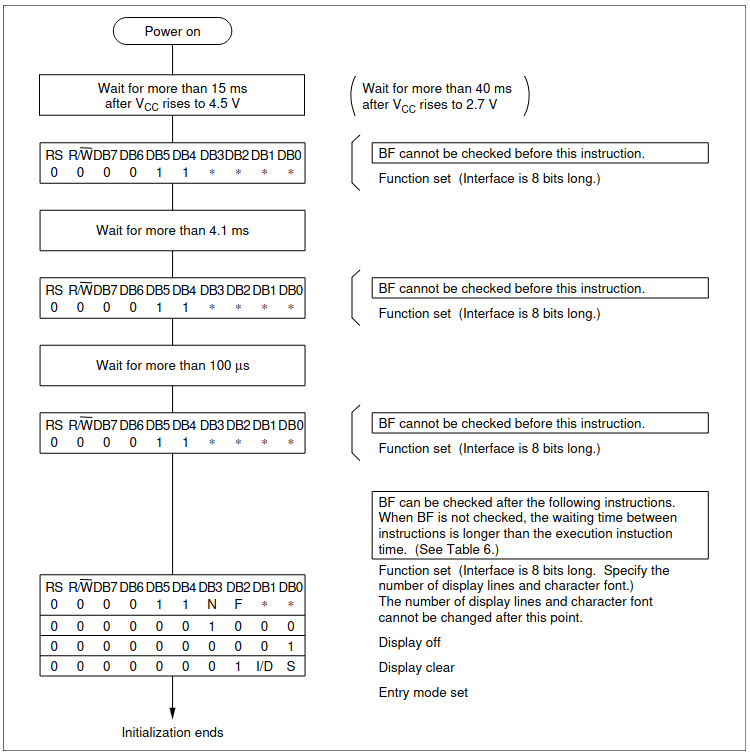
\includegraphics[width=0.6\textwidth]{../images/hd44780_init.png}
	\caption{Khởi tạo HD44780}
\end{figure}

\subsection{Mô đun \acrshort{i2c} PCF8574}

\acrshort{i2c} là một chuẩn được phát triển bởi Philips. Nó là một giao thức 2 dây chậm với tốc độ có thể lên đến 400 kHz. Nó được sử dụng rộng rãi trong hệ thống nhúng. Một số thiết bị sử dụng biến thể không đạt được yêu cầu của \acrshort{i2c} nên có thể được gọi bằng tên khác như TWI hoặc IIC.

SMBus (System Management Bus) dựa trên giao thức \acrshort{i2c} được sử dụng rộng rãi trong hệ thống máy tính. Rất nhiều thiết bị \acrshort{i2c} có thể hoạt động trên SMBus như \acrshort{i2c} EEPROMs và một số chip theo dõi phần cứng.

Trong một bus \acrshort{i2c}, có thể có một hay nhiều master chip được kết nối tới một hay nhiều slave chip.


\begin{figure}[H]
	\centering
	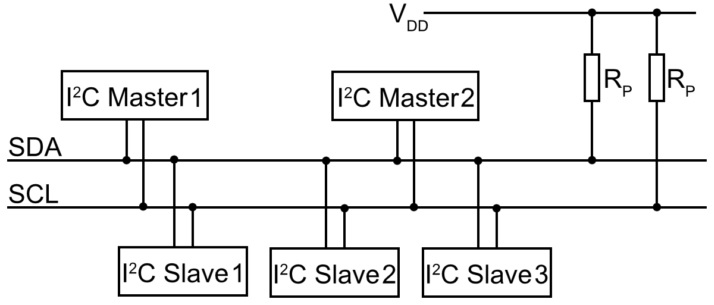
\includegraphics[width=0.6\textwidth]{../images/I2C-Bus-Layout.jpg}
	\caption{\acrshort{i2c} bus}
\end{figure}


Master chip là thiết bị kết nối tới slave. Trong nhân linux, master chip được gọi là một adapter hoặc bus. Các trình điều khiển của adapter nằm trong thư mục con drivers/i2c/busses.

Một algorithm chứa mã có thể sử dụng để cài đặt nhiều loại I2C adapter. Mỗi adapter driver có thể phụ thuộc vào một algorithm driver trong thư mục con drivers/i2c/algos hoặc chứa mã cho riêng nó.

Một slave chip là nút thực hiện giao tiếp khi có yêu cầu của master. trong Linux, nó được gọi là client. Client driver được lưu trong thư mục nào phụ thuộc vào các chức năng mà nó cung cấp, ví dụ như trong drivers/media/gpio cho thiết bị mở rộng GPIO.


Để đơn giản hóa việc điều khiển một thiết bị sử dụng nhiều GPIO, module mở rộng chân sử dụng kết nối nối tiếp sẽ giúp đơn giản hóa việc kết nối và tiết kiệm số chân GPIO. PCF8574 sử dụng giao tiếp \acrshort{i2c} có 8 địa chỉ có thể thay đổi cứng. Địa chỉ mặc định là 0x27 và có 8 chân GPIO song song. 

Việc đọc 8 chân GPIO có thể thực hiện bằng việc đọc 8 bit từ module PCF8574, tương tự, ghi vào 8 chân GPIO được thực hiện bằng việc ghi 8 bit tương ứng.


\chapter{PHÂN TÍCH - THIẾT KẾ}
\section{Mô tả bài toán}
\subsection{Yêu cầu chức năng}
Màn hình LCD1602 có nhiều chức năng phục vụ việc hiển thị văn bản. Vì vậy, thiết bị có một số yêu cầu chức năng trong hình \ref{func-req} bao gồm các chức năng điều khiển con trỏ, chức năng điều khiển các chức năng hiển thị và nội dung hiển thị.
\begin{figure}[H]
	\centering
	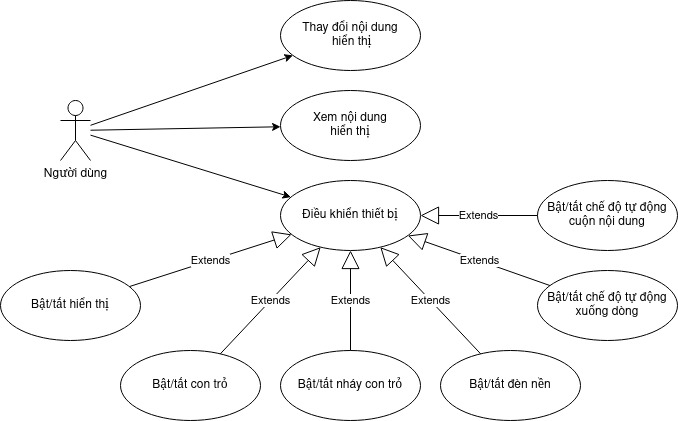
\includegraphics[width=0.8\textwidth]{../images/linux-usecase.jpg}
	\caption{BIểu đồ usecase}
	\label{func-req}
\end{figure}
\subsection{Yêu cầu phi chức năng}
Hệ thống cần đạt được một số yêu cầu phi chức năng:

\begin{itemize}
	\item Hệ thống cần đáp ứng nhanh, xử lý nhanh tránh trường hợp người dùng chờ quá lâu sau khi nhập.
	\item Số ký tự tối đa được nhập dưới 100 ký tự, nếu vượt quá khoảng hiển thị của màn hình LCD1602, thực hiện thuật toán cuộn trang để hiển thị các ký tự.
	\item Thông tin hiển thị rõ ràng, chính xác.
\end{itemize}
\section{Sơ đồ khối}
Phần cứng bao gồm thiết bị và máy tính điều khiển. Trong đó thiết bị bao gồm 2 khối màn hình và mạch Raspberry Pi 3. Trong mỗi thành phần lại bao gồm các mô đun phần mềm và phần cứng khác nhau (Hình \ref{block-diagram}). Khối máy tính điều khiển của người dùng thực hiện chạy chương trình điều khiển và giao tiếp với mạch Raspberry Pi qua dịch vụ SSH. Tại Raspberry Pi, dịch vụ SSH chạy lệnh tương tác với hệ thống Sysfs của trình điều khiển thiết bị màn hình để điều khiển hoạt động của màn hình. Khối màn hình bao gồm mô đun PCF8574 và màn hình LCD1602 sẽ hoạt động theo sự điều khiển của trình điều khiển trên mạch Raspberry Pi.

\begin{figure}[H]
	\centering
	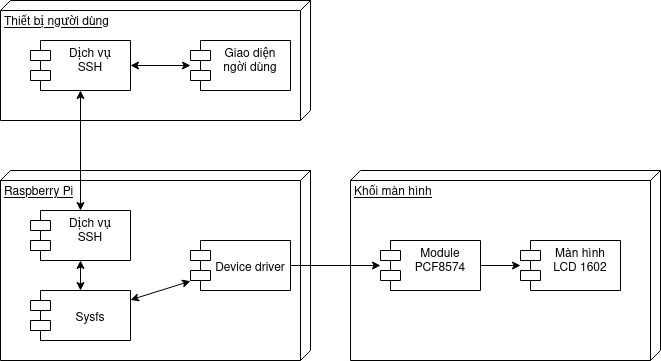
\includegraphics[width=0.8\textwidth]{../images/linux-component.jpg}
	\caption{Sơ đồ khối hệ thống}
	\label{block-diagram}
\end{figure}
\section{Trình điều khiển thiết bị}
Trình điều khiển thiết bị (Driver) là thành phần phần mềm chính của thiết bị. Hoạt động của mô đun này được mô tả trong hình \ref{driver-block}. Luồng điều khiển liên tục chạy và thay đổi trạng thái màn hình tùy theo dữ liệu người dùng nhập như khi người dùng thay đổi nội dung, thay đổi trạng thái màn hình hay khi thực hiện cuộn văn bản.

Dữ liệu driver được cập nhật bởi người dùng thông qua hệ thống sysfs. Dữ liệu trạng thái sau khi cập nhật sẽ được cập nhật bởi luồng điều khiển và hiển thị trên màn hình LCD1602.

\begin{figure}[H]
	\centering
	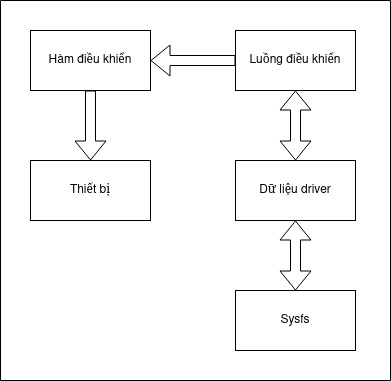
\includegraphics[width=0.8\textwidth]{../images/driver.jpg}
	\caption{Sơ đồ khối của trình điều khiển thiết bị}
	\label{driver-block}
\end{figure}

Luồng điều khiển chính được mô tả trong hình \ref{main-thread}. Do luồng trong không gian nhân không thể kết thúc một cách tự động hoặc kết thúc từ luồng khác mà chỉ có thể gửi tín hiệu kết thúc đến nó nên các câu lệnh phải được đặt bên trong vòng lặp kiểm tra trạng thái kết thúc. Bên trong vòng lặp, thực hiện lấy dữ liệu hiển thị và gọi hàm hiển thị tương ứng nếu dữ liệu có sự thay đổi. Sau đó gọi hàm làm mới dữ liệu và tạm dừng luồng trong 1 giây để chuyển sang vòng lặp tiếp theo.

\begin{figure}[H]
	\centering
	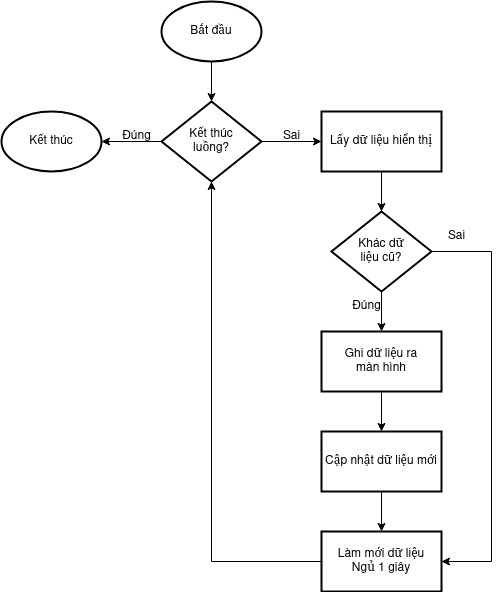
\includegraphics[width=0.8\textwidth]{../images/driver-work-thread.jpg}
	\caption{Hoạt động của luồng điều khiển chính}
	\label{main-thread}
\end{figure}

Người dùng thực hiện thao tác với màn hình qua hệ thống file ảo của sysfs bằng việc đọc hoặc ghi vào chúng. Thao tác này có thể thực hiện trực tiếp trên shell nên có thể lập trình giao tiếp qua các dịch vụ từ xa như Secure Shell. Các file nằm trong đường dẫn /sys/kernel/pcf\_lcd.
\begin{table}[H]
	\centering
	\caption{Danh sách file sysfs}
	\begin{tabular}{|c|c|}
		\hline
		\textbf{Tên file} & \textbf{Chức năng}\\
		\hline
		content & đọc hoặc ghi nội dung hiển thị\\
		line1 & đọc nội dung dòng 1\\
		line2 & đọc nội dung dòng 2\\
		scroll & bật/tắt chế độ cuộn văn bản\\
		auto\_newline & bật/tắt chế độ tự động xuống dòng\\
		backlight & bật/tắt đèn nền \\
		cursor & bật/tắt con trỏ \\
		blink & bật/tắt nháy con trỏ\\
		display & bật/tắt hiển thị\\
		\hline		
	\end{tabular}
\end{table}
\section{Giao diện dồ họa}
Giao diện đồ họa được sử dụng nhằm điều khiển hoạt động của màn hình LCD1602. Các thành phần trong giao diện tương ứng với các chức năng của driver bao gồm:
\begin{itemize}
	\item Các chức năng bật/tắt: Sử dụng checkbox.
	\item Thay đổi nội dung: Sử dụng một khung nhập văn bản và nút nhấn Submit.
	\item Thực hiện chức năng kết nối: Sử dụng một dòng input để nhập Hostname và nút nhấn Login, thực hiên kiểm tra đăng nhập vào thiết bị với người dùng Root qua kết nối SSH.
\end{itemize}
\chapter{XÂY DỰNG HỆ THỐNG}
\section{Triển khai phần cứng}
Phần cứng máy tính nhúng được sử dụng là mạch phát triển Raspberry Pi 3 với sơ đồ ra chân như hình \ref{rpi3-pinout}. 
\begin{figure}[H]
	\centering
	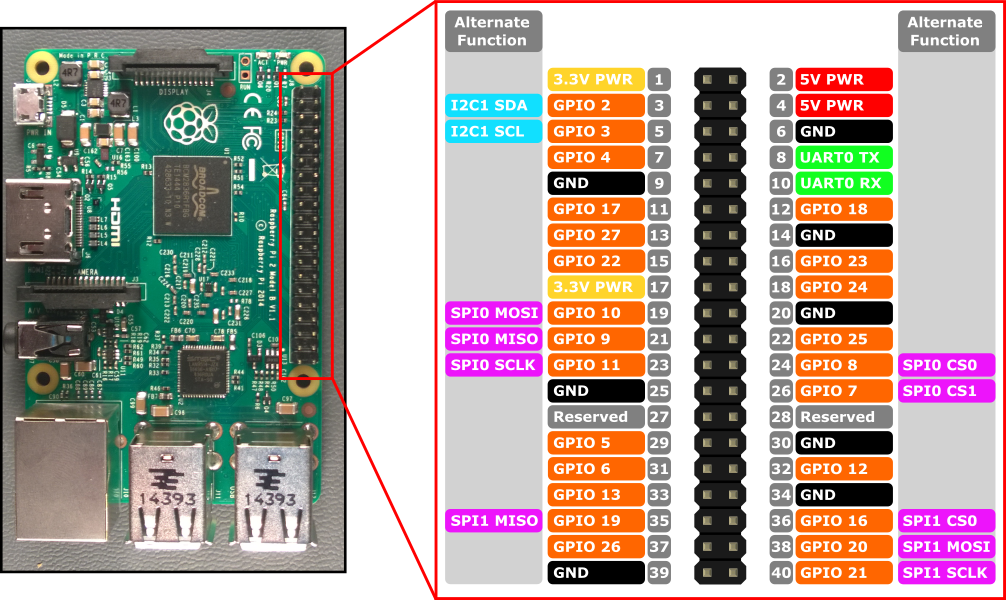
\includegraphics[width=0.8\textwidth]{../images/rp3_pinout.png}
	\caption{Sơ đồ ra chân các ngoại vi của Raspberry Pi}
	\label{rpi3-pinout}
\end{figure}

Mô đun PCF8574 cho màn hình LCD1602 được kết nối tới Raspberry Pi qua ngoại vi I2C1 duy nhất với 4 dây nối tương ứng trong bảng \ref{wiring}.

\begin{table}[H]
	\centering
	\caption{Sơ đồ nối dây giữa Raspberry Pi và mô đun PCF8574}
	\begin{tabular}{|c|c|}
		\hline
		\textbf{Chân Raspberyr Pi} & \textbf{Chân PCF8574}\\
		\hline
		5V & VCC\\
		GND & GND\\
		GPIO3 & SCL\\
		GPIO2 & SDA\\
		\hline
	\end{tabular}
	\label{wiring}
\end{table}

\section{Triển khai driver}
Driver được triển khai trên nhiều file. File lcd\_data.h chứa dữ liệu cho hoạt động điều khiển của driver (nội dung hiển thị, các dữ liệu điều khiển hiển thị, cuộn trang, ...).  File lcd\_sysfs.h giúp xuất dữ liệu driver và thay đổi dữ liệu driver theo yêu cầu của người dùng sử dụng hệ thống sysfs. File lcd\_i2c\_client.h chứa các hàm tương tác với thiết bị như điều khiển đèn nền, điều khiển cuộn trang hay thay đổi dữ liệu. File pcf\_lcd.c là file chính của driver, thực hiện khai báo driver, khởi tạo luồng điều khiển, các hàm probe, remove.

Trong luồng điều khiển hoạt động của driver, thực hiện liên tục lấy dữ liệu hiển thị cho màn hình. Dữ liệu này có thể thay đổi sau mỗi lần lặp do dữ liệu mới được cập nhật hoặc sau khi làm mới dữ liệu, ở chế độ cuộn văn bản, dữ liệu hiển thị bị dịch chuyển sang ký tự khác. Sơ đố luồng điều khiển được thể hiện trong hình \ref{main-thread}.

Khi khai báo driver, thực hiện tạo đối tượng struct i2c\_driver trong đó bao gồm các trường probe\_new cho việc khởi tại thiết bị, .remove cho việc 	gỡ bỏ thiết bị, .id\_table là đối tượng struct i2c\_device\_id cho thiết bị, .of\_match\_table là struct of\_device\_id chứa thông tin tên thiết bị tương thích với driver được lưu trong device tree.
\lstinputlisting[firstline=66, firstnumber=66, lastline=109]{../../pcf_lcd.c}

Việc làm mới dữ liệu được thực hiện liên tục để phục vụ mục đích hiển thị dữ liệu mới từ người dùng hoặc phục vụ mục đích cuộn nội dung. Hàm làm mới dữ liệu được khai báo bên trong file chứa dữ liệu.
\lstinputlisting[firstline=8,firstnumber=8, lastline=23]{../../lcd_data.h}
\lstinputlisting[firstline=143,firstnumber=143, lastline=176]{../../lcd_data.h}

\section{Triển khai giao diện đồ họa}
Giao diện đồ họa được thực hiện thông qua bộ công cụ QT sử dụng ngôn ngữ QML và Rust. Kết nối SSH được thực hiện thông qua phần mềm của hệ thống. Với mỗi thao tác như nhấn vào checkbox hay thay đổi nội dung hiển thị, màn hình sẽ thực hiện thao tác tương ứng.
\begin{figure}[H]
	\centering
	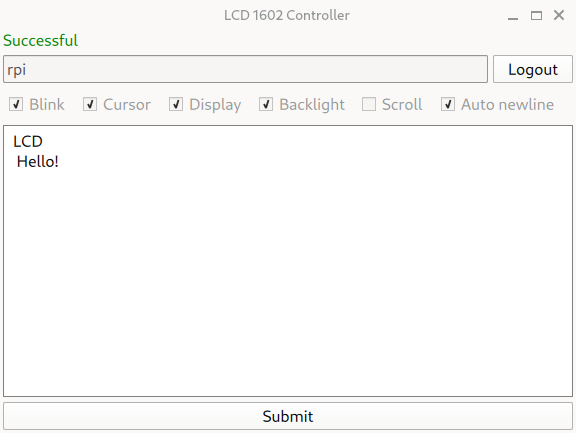
\includegraphics[width=0.8\textwidth]{../images/gui.png}
	\caption{Giao diện đồ họa}
\end{figure}
\section{Thử nghiệm thiết bị}
Sau khi thực hiện kiểm tra kết nối bằng cách nhấn login, thực hiện thay đổi nội dung hiển thị và nhấn submit trên giao diện (Hình \ref{gui-change-content}), màn hình thiết bị sẽ thực hiên hiển thị nội dung với chế độ tương ứng (Hình \ref{dev-change-content}).
\begin{figure}[H]
	\centering
	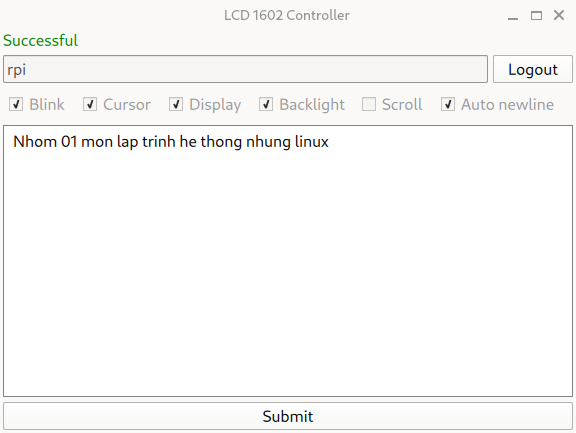
\includegraphics[width=0.8\textwidth]{../images/Screenshot from 2023-06-10 11-05-54.png}
	\caption{Thực hiện đổi nội dung hiển thị}
	\label{gui-change-content}
\end{figure}
\begin{figure}[H]
	\centering
	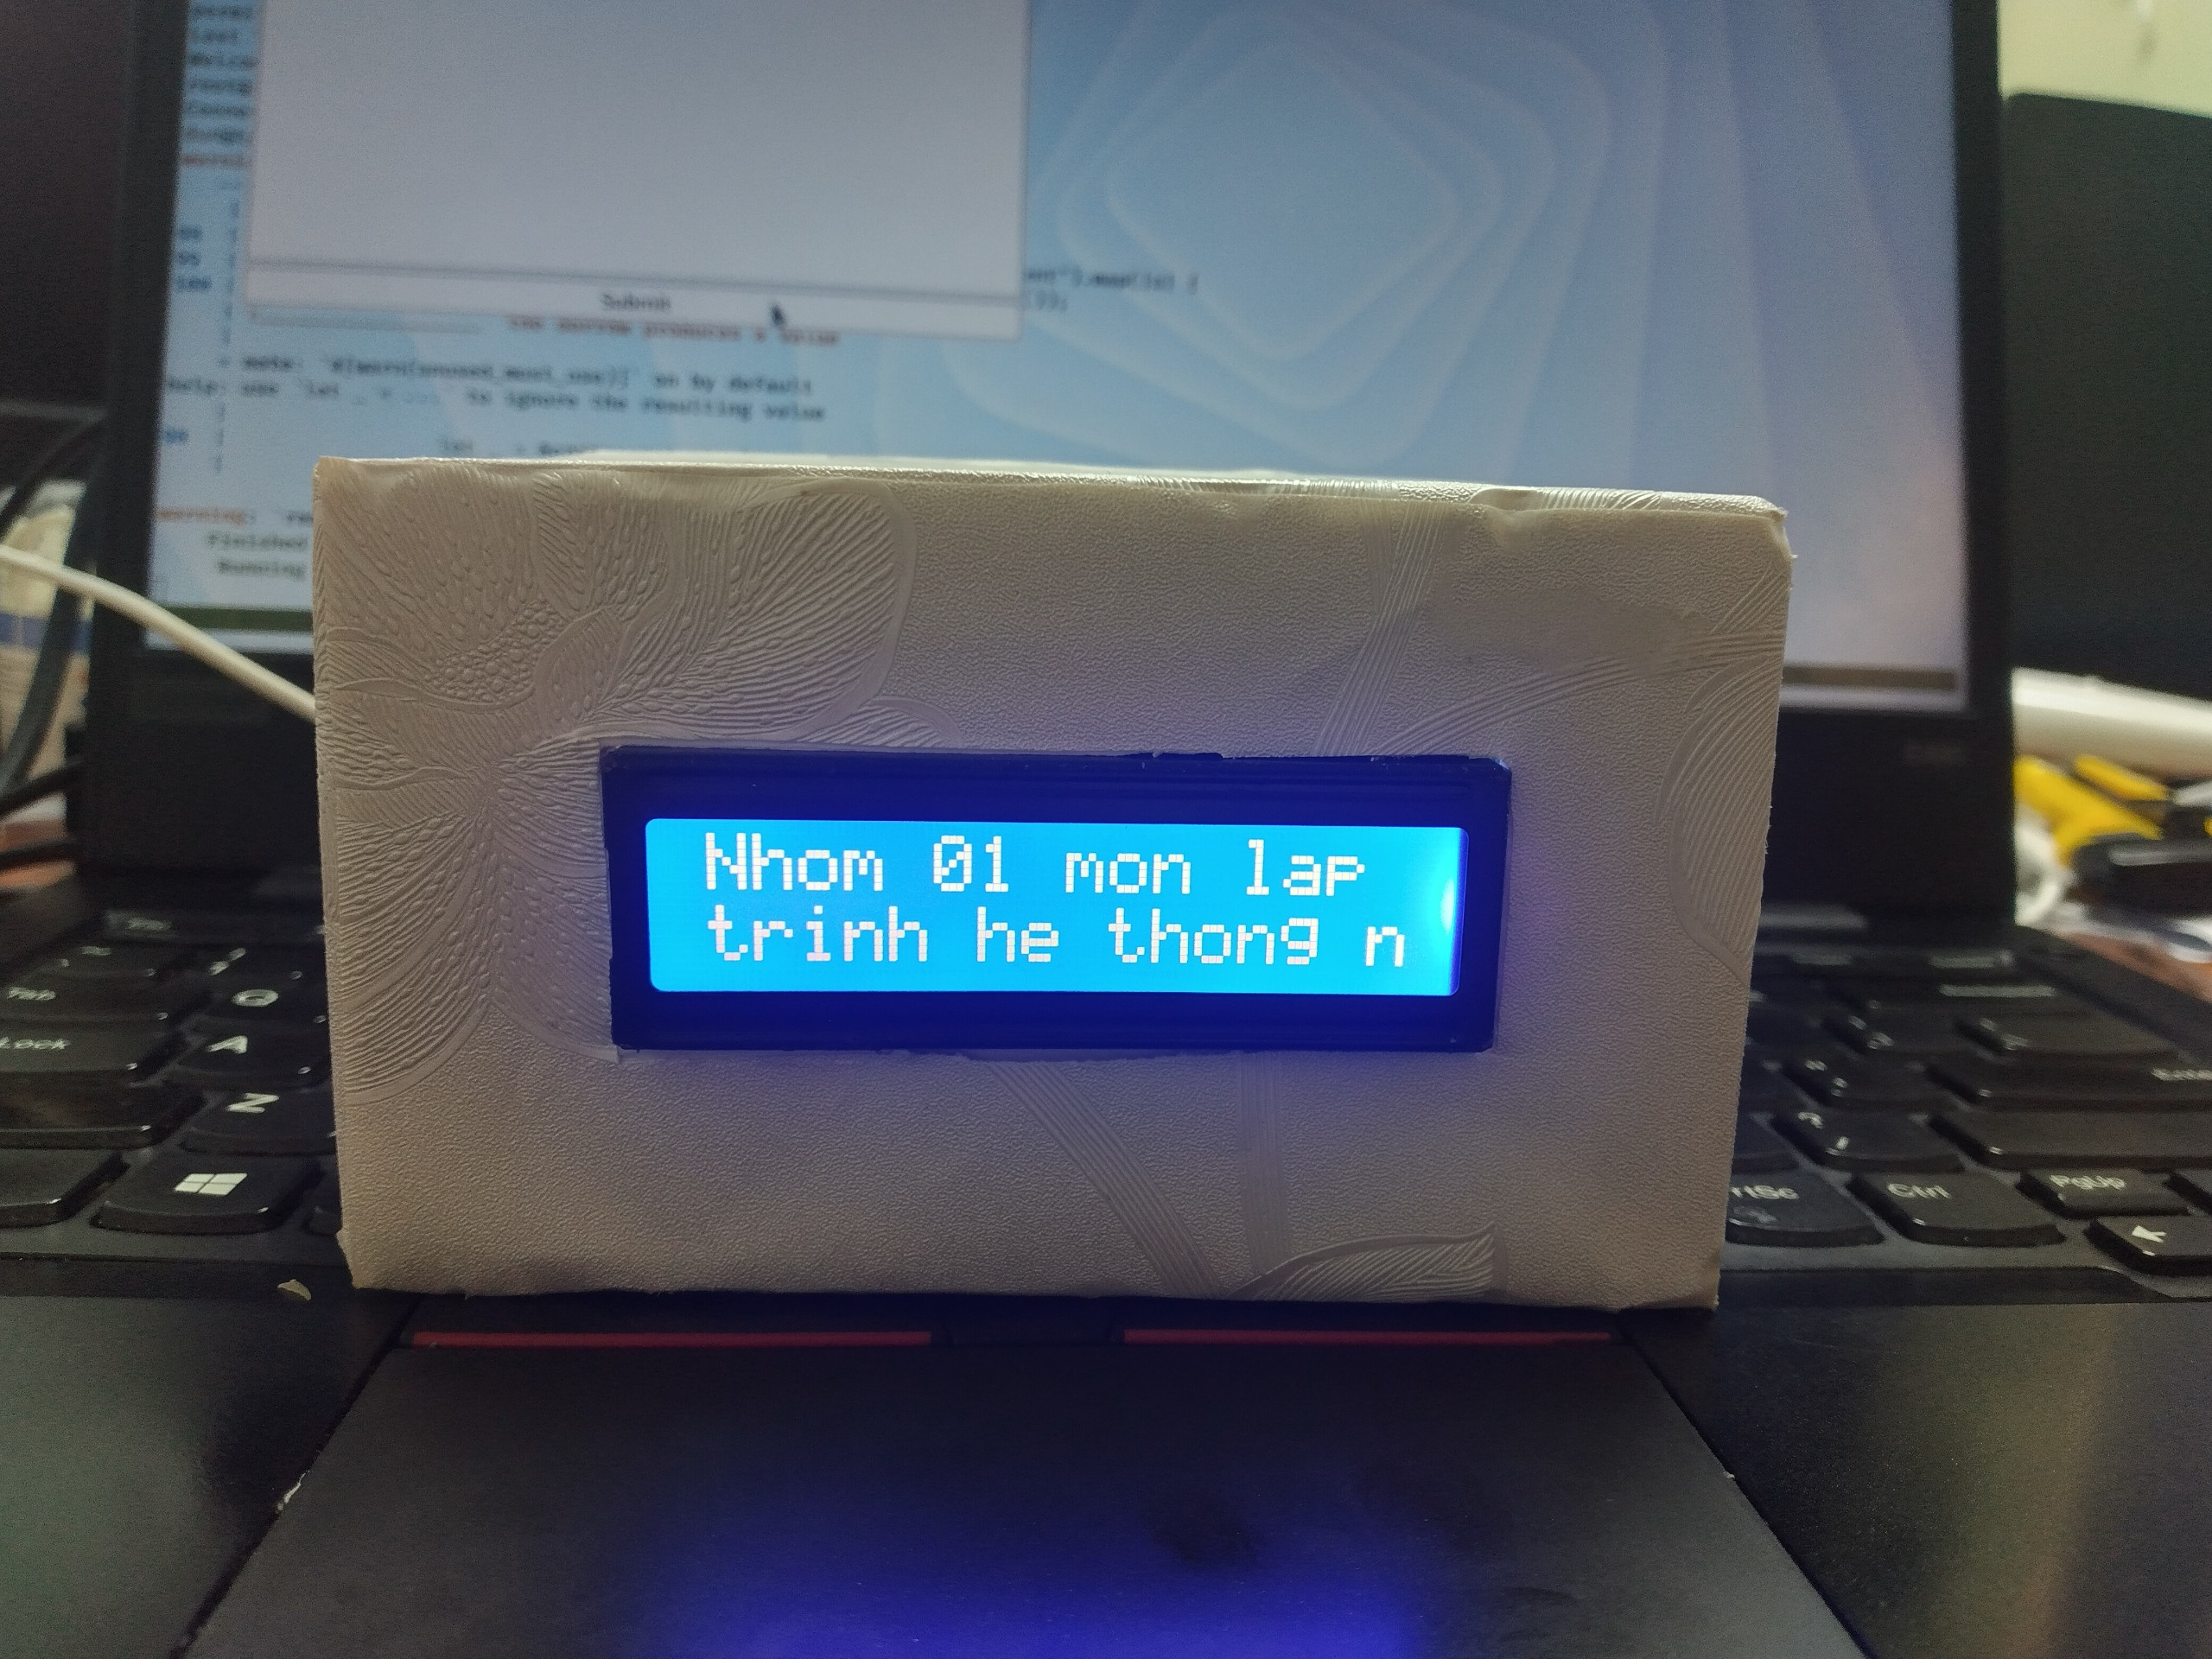
\includegraphics[width=0.8\textwidth]{../images/man-hinh-thay-doi.jpg}
	\caption{Màn hình hiển thị sau khi đổi nội dung}
	\label{dev-change-content}
\end{figure}
\section{Nhận xét}
Hệ thống đã đảm bảo đầy đủ theo các chức năng như đề ra trong đề tài. Hệ
thống đã được xây dựng với các thiết bị phần cứng và phần mềm đúng như yêu
cầu môn học đưa ra. Nội dung hiển thị chính xác và đầy đủ.
\section{Hạn chế của thiết bị}
Hệ thống đã đạt được mong muốn đề ra nhưng cũng không tránh khỏi những
sai sót. Do hệ thống được phát triển ở mức thực nghiệm nên thiết kế sản phẩm có
sơ sài về mặt kết nối các phần cứng. Đôi khi kết nối chập chờn dẫn đến sai sót
trong hiển thị.
\chapter{KẾT LUẬN}
\section{Kết quả đạt được}
Qua quá trình nghiên cứu các thuật toán, kiến thức liên quan đến linux, trình điều khiển thiết bị, nhóm chúng em đã đạt được một số thành tựu:
\begin{itemize}
	\item Tìm hiểu giao thức, điều khiển thành công việc đọc, ghi dữ liệu qua giao tiếp \acrshort{i2c}.
	\item Tìm hiểu phương pháp phát triển trình điều khiển thiết bị cho thiết bị \acrshort{i2c} trên môi trường linux.
	\item Hiểu phương pháp lập trình nhúng trên Linux, biết thêm phương pháp lập trình giao diện.
\end{itemize}
\section{Phương hướng phát triển và đề xuất}
Bên cạnh những công việc đã đạt được, nhóm cũng có các phương hướng mở rộng đề tài như sau:
\begin{itemize}
	\item Thực hiện hiển thị nội dung thời gian thực trên giao diện đồ họa.
	\item Tối ưu thuật toán để nội dung hiển thị được dễ nhìn hơn.
	\item Thêm các chức năng hiển thị các thông số khác của kernel.
	\item Chỉnh sửa, thêm các thành phần tối ưu cho mục đích truyền nhận dữ liệu.
\end{itemize}

\renewcommand\bibname{TÀI LIỆU THAM KHẢO}

\bibliographystyle{plain}

\bibliography{../essential/refs}

\chapter*{PHỤ LỤC: MÃ NGUỒN CHƯƠNG TRÌNH}

Mã nguồn chương trình được đăng tải trực tuyến tại đường dẫn: \url{https://github.com/dungph/driver-lab}

\end{document}
